\documentclass{article}
\usepackage{amsmath}
\usepackage{mathtools}
\usepackage{graphicx, color}
\graphicspath{{figs/}}

%----------------------------------
%\topmargin      -1.5cm   % read Lamport p.163
%\oddsidemargin  -0.04cm  % read Lamport p.163
%\evensidemargin -0.04cm  % same as oddsidemargin but for left-hand pages
%\textwidth      16.59cm
%\textheight     22.94cm

%\topmargin      -1.5cm   % read Lamport p.163
\oddsidemargin  0.04cm  % read Lamport p.163
\evensidemargin 0.04cm  % same as oddsidemargin but for left-hand pages
\textwidth      15cm
%\textheight     22.94cm

\parskip         7.2pt   % sets spacing between paragraphs
%\parindent         3mm   % sets leading space for paragraphs
%-------------------------------------

\title{ Covariance Matrix Prior distribution \\ On Hierarchical Linear Models }
\author{Ignacio Alvarez}
\date{ Fall 2013 }

\begin{document}
\maketitle 

\vspace{3cm}

\section{Introduction} 

In this work we explore several choices for the covariance matrix prior in a hirerarchical regression model. 
Approcahes .... 
Objetives ....
Aplication description .....



\section{Statistical Models} 
We will deal with linear models using time as the main covariate variable and a response variable changing over time, also the data will be separated in groups (bird species in our example), then $Y_{ts}$ will be the response value for group $s$ at time $t$. 

We want to fit a linear model for each group $Y_ts \sim N(\beta_{1s} + t\beta_{2s}, \sigma_s)$, but we could combine information across groups. The way in what we combine group information is reflected in the prior. We may want to fit a separate prior for each parameter within each group, in this case each group model is completely independent from the rest. 

On the opposite side we could combine all the groups into one set of parameters estimated using all groups information. Finally as a compromise between the previous options we can allows different parameters for each group but all with common prior distribution, i.e. a hierarchical model. 

These options in how combine information across groups can be done independently for $\beta_s=(\beta_{1s}\;\;\beta_{2s})$ or for $\sigma_s$, which lead us to a 9 ways setting up the prior distributions for all the parameters in the model. Table \ref{stmod} presents the basic choices of models we just described, rows of the table are the trhee ways we can combine the groups information for the $\beta_s$ coefficients and the columns represents the same thing but for $\sigma_s$ instead. 
The result are nine models, each of the nine cells in Table \ref{stmod} represents one of those combination. 
 
\begin{table}%
\caption{Basic Model Structure Choices \label{stmod} } 
\begin{tabular}{|l|ccc|} \hline \hline
& same & hierarchical & Different \\ \hline\hline
same  
&$Y_s \sim N(X_s\beta,\sigma^2)$&$Y_s \sim N(X_s\beta,\sigma_s^2)$& $Y_s \sim N(X_s\beta, \sigma_s^2)$ \\
&$\beta\sim N(\mu_0, \Sigma_0)$&$\beta\sim N(\mu_0, \Sigma_0)$&$\beta\sim N(\mu_0, \Sigma_0)$ \\
&$\sigma\sim unif(0, v_0)$ &$\sigma_s\sim invGamma(\alpha_s, \lambda_s)$& $\sigma_s\sim unif(0, v_0)$ \\ 
& & $\alpha_s \sim unif(0,a_0)$, $\lambda_s\sim unif(0,l_0)$ & \\ \hline 
hierarchical 
&$Y_s \sim N(X_s\beta,\sigma^2)$&$Y_s \sim N(X_s\beta,\sigma_s^2)$& $Y_s \sim N(X_s\beta, \sigma_s^2)$ \\
&$\beta_s\sim N(\mu, \Sigma)$&$\beta_s\sim N(\mu, \Sigma)$ & $\beta_s\sim N(\mu,\Sigma)$ \\
& $\mu \sim N(\psi_0, \Psi_0) $ & $\mu \sim N(\psi_0, \Psi_0) $ & $\mu \sim N(\psi_0, \Psi_0) $ \\ 
& $\Sigma \sim invWishart(R_0,d_0)$& $\Sigma \sim invWishart(R_0,d_0)$& $\Sigma \sim invWishart(R_0,d_0)$ \\  
&$\sigma\sim unif(0, v_0)$ &$\sigma_s\sim invGamma(\alpha_s, \lambda_s)$& $\sigma_s\sim unif(0, v_0)$ \\ 
& & $\alpha_s \sim unif(0,a_0)$, $\lambda_s\sim unif(0,l_0)$ & \\ \hline 
different 
&$Y_s \sim N(X_s\beta,\sigma^2)$&$Y_s \sim N(X_s\beta,\sigma_s^2)$& $Y_s \sim N(X_s\beta, \sigma_s^2)$ \\
&$\beta_s\sim N(\mu_0, \Sigma_0)$&$\beta_s\sim N(\mu_0, \Sigma_0)$&$\beta_s\sim N(\mu_0, \Sigma_0)$ \\
&$\sigma\sim unif(0, v_0)$ &$\sigma_s\sim invGamma(\alpha_s, \lambda_s)$& $\sigma_s\sim unif(0, v_0)$ \\ 
& & $\alpha_s \sim unif(0,a_0)$, $\lambda_s\sim unif(0,l_0)$ & \\ \hline\hline
\end{tabular}
\end{table}

Some comments about the models and notation contain in Table \ref{stmod}

\begin{itemize}
	\item All the symbols with ''0'' subscript represent numerical known values not parameters we learn from data, usually these parameter are set to assure the non informativity of the prior. For instance $v_0$, $a_0$ and $l_0$ are the upper limits of uniforms distributions for variance parameter or hyperparameter and then will be set as very high numerical values. 
	\item As example, the first cell in the table is representing a separate regressions for each group with flat priors on all parameters. 
	\item All data models are written in matrix form. If we have observations for the times $t=1, 2, \ldots, T$, then  the vector $Y_s$ represent all observations for group $s$, $Y_s =  (Y_1,Y_2,\dots,Y_T)^{'}$. Also $X_s$ is a $T\times 2$ matrix which its $t$ht row is $X_st = [1\;t]$. This can be extended to add a quadratic term to the model. 
	\item Parameters are also in matrix form, so $\beta_s$ and $\mu$ are two-dimensional vectors representing intercept and slope for group $s$ and its prior mean, while $Sigma$ is the 2$\times$2 $\beta_s$ covariance matrix. In case we add a quadratic term in the model this vectors will be 3 dimensional. 
	\item Note that $\mu_0$ and $Sigma_0$ are numerical values not parameters, so they are not vector or matrices just scalar known values. 
	\item We choose a uniform prior on standar deviation scale for $\sigma_s$ and its related hyperparameters, this is following Gelman recommendation on REF, but we could set a different options as inverse gamma flat prior as recomended on REF or an improper prior. 
	\item The inverse Wishart prior for the covariance matrix will be the main interest in this work, we will study advantage and disadvantages of this choice and explore the alternatives to it. 
\end{itemize}
 


\section{ Bird Populations modelling} 
According to (REF, Etterson) one of the basic research goals in Ecology consist on understand the distribution and abundance of the animal population. In this work, the particular goal will be to explore alternatives to model the time trends in Western Great Lakes Birds population over 1994 to 2011. 

\subsection{Data description}
The data source for this study came from ``an extensive, long-term monitoring program with over 1600 off-road sampling points designed to track regional population trends and investigate the response of forest birds to regional land use patterns''(REF:). 

This monitoring program is carry out by Natural Resources Research Institute (University of Minnesota Duluth) with the objective of ``sustain forest resources and bird diversity in western Great Lakes forests'' (REF: ). 

For this report in particular the dataset which will be used in this report consist in the yearly bird count for 73 species on three National Forest from 1995 to 2013. There are several interesting covariate that are measured in the sampling procedure, however most of them are site characteristics at the moment when the sampling was done, therefore they are not so meaningfully when we consider yearly aggregated data.  

We can see a first look of the data in Figure \ref{figtr}, where the total bird count per year is plotted for all three forest. We can see Superior is consistently over all years the forest with more bird counts (why? is bigger ?) reaching 10000 counts on three time during the monitoring period. The others two forest, Chequamegon and Chippewa show a similar trend in the total bird count. 


Overall, it seems to be a first sub-period from 1995 to 2003 where the total bird count is increasing every year but from that this increment stop. From 2003 on Superior forest it seem to oscillate around a little more than 8000 birds while for Chequamegon the count are getting smaller each year. 

\begin{figure}[h!]
\centering
\includegraphics[scale=.4, angle=-90]{rawtrend.ps}
\caption{Raw trend in the data \label{figtr} }
\end{figure}

There is a big variability of the counts among species. Table \ref{t1} presents the total bird count on year 2007 for the most abundant species, (just to compare it with the on line annual report). We can see that OVEN and REVI are very abundant species among all forest. 

However the structure of abundant is different on each forest. Species like NAWA and WTSP are abundant only in Superior forest, while VEER it is only abundant for Chippewa. In order to model the species count along time it might be better to work separately by forest (at least in a initial steps).  

% latex table generated in R 3.0.2 by xtable 1.7-1 package
% Wed May 28 11:30:44 2014
\begin{table}[ht]
\centering
\caption{Total counts on 2007 for the 10 most abundant species} 
\label{count07}
\begin{tabular}{llrrr}
  \hline
Specie & Abbrev & Chequamegon & Chippewa & Superior \\ 
  \hline
Ovenbird & OVEN & 1003 & 835 & 1168 \\ 
  Red-eyed Vireo & REVI & 823 & 997 & 771 \\ 
  Nashville Warbler & NAWA & 240 & 348 & 867 \\ 
  Blue Jay & BLJA & 222 & 199 & 230 \\ 
  Chestnut-sided Warbler & CSWA & 211 & 330 & 375 \\ 
  White-throated Sparrow & WTSP & 180 & 387 & 940 \\ 
  Hermit Thrush & HETH & 175 & 249 & 265 \\ 
  American Robin & AMRO & 156 & 102 & 154 \\ 
  Least Flycatcher & LEFL & 155 & 368 & 120 \\ 
  Veery & VEER &  91 & 402 & 264 \\ 
   \hline
\end{tabular}
\end{table}


\subsection{Initial models} 

As a starting point we consider separate regression equations for each specie and forest, a model for one species is represented on equation \ref{mod1}. 
\begin{eqnarray}
\nonumber Y_{ts} &=&  \beta_{0s} + \beta_{1s}t + \beta_{2s}t^2 + \epsilon_{ts}  \\
\epsilon_{ts} &\sim& N(0,\sigma_{s}^2)
\label{mod1}
\end{eqnarray}
where $Y_{ts}$ represent the average bird count on year $t$ in the forest $f$ for the specie $s$. From a bayesian point of view this consist in a hierarchical Normal model where $Y_{ts}\vert (\beta_{0s},\beta_{1s},\beta_{2s},\sigma_{s}) \sim N(\beta_{0s}+\beta_{1s}t+\beta_{2s}t^2, \sigma_{s})$ and all parameters are independents with flat priors and different values for each species. 

There are 73 species and we fit the model \ref{mod1} for 3 different forests there are 219 individual species regression models in total. In addition, we consider two variants from \ref{mod1}. First, it is not clear that we need to include a quadratic term in the regression term so we may consider a simple regresion only. Second, it is common to log transform the average counts. So, for each species we consider 4 models including two types of response variable (in logs and average count) and two set of predictors (quadratic and only linear). 
 
Along this report the parameters of interest will be the regression slope for each species.  Figure \ref{histm1} presents these slopes median for each species on every scenario we run for all three forest. There are 12 panels, each row represent one forest (Chequamegon, Chippewa and Superior) and each column represent one type of model (linear in logs, quadratic in logs, linear with counts and quadratic with counts).  
\begin{figure}[h!]
\centering
\includegraphics[scale=.5, angle=-90]{hist_m1.ps}
\caption{Species slopes from model \ref{mod1} . \label{histm1}}
\end{figure}

The slopes histograms are similar on the 3 forest within each model type. The model with the log transformed response seem to present a more symmetric distribution of the slopes, when we use the average counts most of the slopes are very close to zero value except for a few species with high slope values. 

Next, we explore the bivariate relation among the coefficients within each regression. With this in mind we can see a scatter matrix of the estimated coefficients in Figure \ref{pairss1}. The main point to see here is a negative relation between the slope and the quadratic term for all forest, is .67, .82 and .83 on Chequamegon, Chippewa and Superior respectively. (KAISER Dix it: while polynomials are wonderfully flexible functions for describing data patterns, they do not lend themselves to interpretation of coefficient values -different combinations of constant, linear, and quadratic terms can lead to quite similar functions over a finite range of covariate values) 

\begin{figure}[h!]
\centering
\includegraphics[scale=.6, angle=-90]{scat_m1.ps}
\caption{Bivariate relation among coefficients of model \ref{mod1}. \label{pairs1}}
\end{figure}
Also, there is a negative relation between between intercept and variance, specially for Chequamegon and Chippewa forest. Maybe the main message for this plot is that we should not treat this parameters as independent and try to include their dependence into the model we are fitting. 





%\nonumber log(Y_{tfs}) &=&  \beta_{0fs} + \beta_{1fs}t + \beta_{2fs}t^2 + \epsilon_{tfs}  \\
%\beta_{fs} &\sim& N \left( \left[ \begin{array}{c}
    %\beta_{0f}   \\ 
    %\beta_{1f}  \\ 
    %\beta_{2f}  
%\end{array} \right],   \Sigma_f \right) \\ 
%\epsilon_{tfs} &\sim& N(0,\sigma_f^2)
%\label{mod2}
%\end{eqnarray}
%
%where the matrix $\Sigma$ is formed as $(\Sigma)_{ij}=\rho_{ij}\sigma_i\sigma_j$ when $i\neq j$ and $(\Sigma)_{ii}=\sigma_i^2$ on the diagonal, having 6 parameter in total.     
%
%\begin{eqnarray}
%\nonumber Y_{tfs} &=&  \beta_{0fs} + \beta_{1fs}t + \beta_{2fs}t^2 + \epsilon_{tfs}  \\
%\nonumber \beta_{fs} &=& \left(\begin{array}{c}
    %\beta_{0fs}   \\ 
    %\beta_{1fs}  \\ 
    %\beta_{2fs}  
%\end{array}\right) \sim N(\mu_f, \Sigma_{f}) \\
%\nonumber \mu \sim N(0, 100) \\
%\nonumber \Sigma_{f}  &\sim& p(\Sigma) \\ 
%\nonumber \epsilon_{tfs}  &\sim& N(0,\sigma_{\epsilon}^2) \\
%\sigma_{s}^2  &\sim& inv-gama(\alpha,\gamma) \\
%\label{mod.wish}
%\end{eqnarray}
%

%% latex table generated in R 2.15.1 by xtable 1.7-0 package
% Tue Oct 22 17:27:27 2013
\begin{table}[ht]
\begin{center}
\begin{tabular}{llrrr}
  \hline
forestN & par & 2.5\% & 50\% & 97.5\% \\ 
  \hline
Chequamegon & mu[1] & -2.716 & 13.269 & 70.273 \\ 
  Chequamegon & mu[2] & -2.725 & 18.522 & 95.671 \\ 
  Chequamegon & mu[3] & 0.007 & 20.791 & 96.131 \\ 
  Chequamegon & Sigbe[1,1] & -1.357 & 0.027 & 0.778 \\ 
  Chequamegon & Sigbe[2,1] & -1.176 & 0.470 & 1.207 \\ 
  Chequamegon & Sigbe[2,2] & -1.354 & -0.014 & 0.768 \\ 
  Chequamegon & Sigbe[2,3] & -9.309 & 27.471 & 69.695 \\ 
  Chequamegon & Sigbe[3,1] & -9.317 & 0.542 & 14.343 \\ 
  Chequamegon & Sigbe[3,3] & -1.205 & -0.007 & 1.199 \\ 
  Chippewa & mu[1] & -2.958 & 14.508 & 72.993 \\ 
  Chippewa & mu[2] & -2.980 & 18.456 & 96.242 \\ 
  Chippewa & mu[3] & 0.017 & 20.513 & 97.279 \\ 
  Chippewa & Sigbe[1,1] & -1.133 & 0.036 & 0.706 \\ 
  Chippewa & Sigbe[2,1] & -1.012 & 0.350 & 1.009 \\ 
  Chippewa & Sigbe[2,2] & -1.129 & -0.011 & 0.706 \\ 
  Chippewa & Sigbe[2,3] & -10.593 & 29.814 & 72.811 \\ 
  Chippewa & Sigbe[3,1] & -10.594 & 0.390 & 14.485 \\ 
  Chippewa & Sigbe[3,3] & -1.055 & -0.005 & 1.052 \\ 
  Superior & mu[1] & -3.369 & 13.567 & 71.255 \\ 
  Superior & mu[2] & -3.355 & 19.403 & 96.121 \\ 
  Superior & mu[3] & 0.000 & 21.161 & 97.159 \\ 
  Superior & Sigbe[1,1] & -1.352 & 0.009 & 0.215 \\ 
  Superior & Sigbe[2,1] & -0.853 & 0.273 & 0.951 \\ 
  Superior & Sigbe[2,2] & -1.391 & -0.018 & 0.220 \\ 
  Superior & Sigbe[2,3] & -10.627 & 27.807 & 71.247 \\ 
  Superior & Sigbe[3,1] & -10.104 & 0.302 & 13.882 \\ 
  Superior & Sigbe[3,3] & -0.817 & -0.001 & 0.932 \\ 
   \hline
\end{tabular}
\caption{Wishar Prior model}
\end{center}
\end{table}


\begin{figure}[h!]
\centering
\includegraphics[scale=.6, angle=-90]{slp_bet.ps}
\caption{ Slope estimates within each type of variance model}
\end{figure} 




%%%%%%%%%%%%%%%%%%%%%%%%%%%%%%%%%%%%%%%%%%%%%%%%%%%%%%%%%%%%%%%%%%%%%%%%
\end{document}